\section{SpiderMonkey Results}

\begin{figure*}[t]
  \centering
  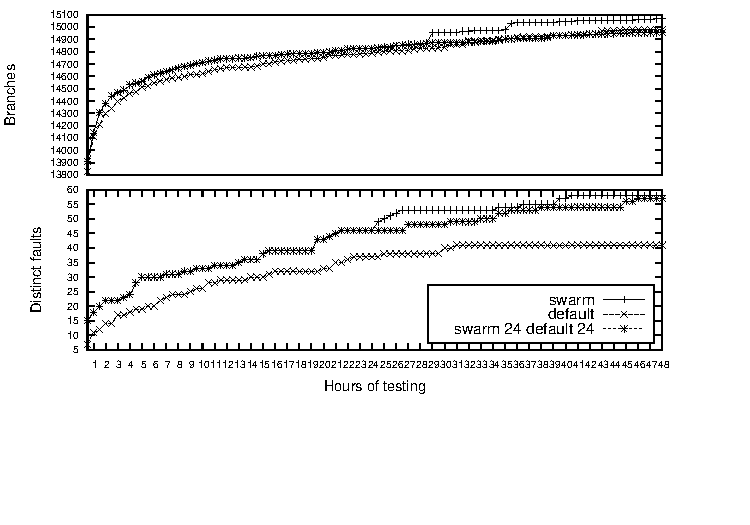
\includegraphics[width=\textwidth]{../graphs/SpiderMonkey/js16}
  \vspace{-1.3in}
  \caption{SpiderMonkey 1.6 Results}
  \label{fig:smonkey16}
\end{figure*}

\begin{figure*}
  \centering
  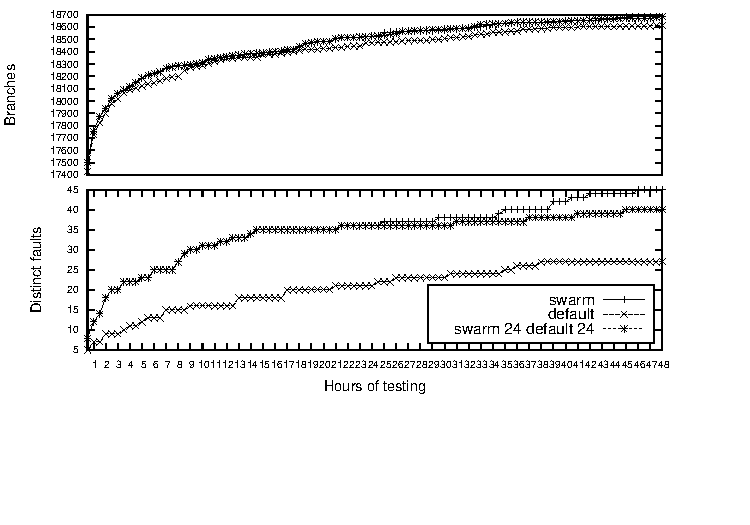
\includegraphics[width=\textwidth]{../graphs/SpiderMonkey/js17}
  \vspace{-1.5in}
  \caption{SpiderMonkey 1.7 Results}
  \label{fig:smonkey17}
\end{figure*}

\begin{figure*}[b]
  \centering
  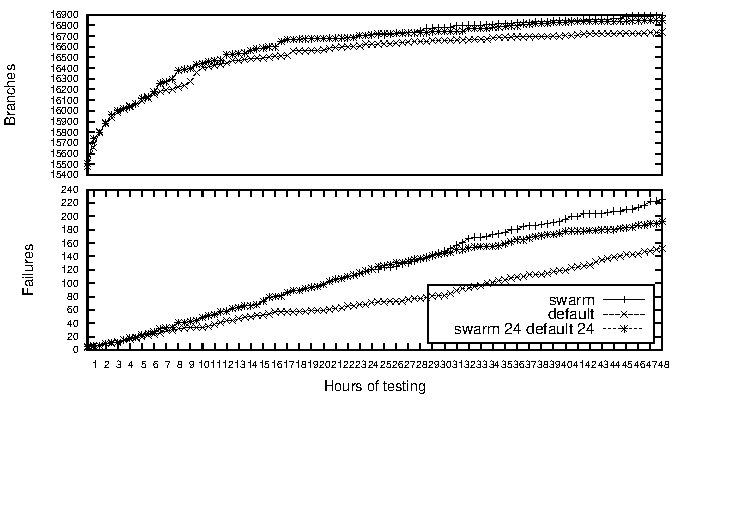
\includegraphics[width=\textwidth]{../graphs/SpiderMonkey/js185}
  \vspace{-1.5in}
  \caption{SpiderMonkey 1.8.5 Results:  Note that this graph shows failures rather than faults.}
  \label{fig:smonkey185}
\end{figure*}

Figures \ref{fig:smonkey16}-\ref{fig:smonkey185} show a comparison
between swarm testing and a default strategy for Mozilla's
SpiderMonkey JavaScript engine, for release versions 1.6, 1.7, and
1.8.5.  Tests were generated using the last public version of the {\tt
jsfunfuzz} JavaScript fuzzing tool~\cite{jsfunfuzz}, both in its
original form and modified to perform swarm testing.  The modification
of {\tt jsfunfuzz} to perform swarm testing was extremely simple.
First, the source code was reformatted with a regular expression to
place individual choices in the random selectors on separate lines.
Second, the reformatted code was ``swarmed'' by a 30 line python
script that removed items in each random choice, with 50\% probability
for each removal.  We estimate that this process took perhaps 30
minutes for a developer unfamilliar with either the {\tt jsfunfuzz}
code or the JavaScript language.

\subsection{Experimental Procedure}

Tests were generated in 30 minute budget runs, and coverage and
faults or failures were computed for each 30 minute run.  The graphs
show cumulative branch coverage and faults or failures for 48 hours of
testing.  In addition to a pure-swarm and pure-default strategy, we
also show results for a strategy that performs swarm testing for 24
hours, then switches to the default configuration, in the hope that
this will explore behaviors hard to reach under swarm.

Distinct faults for versions 1.6 and 1.7 were estimated by using
historical repository data; all faults detected for these versions
were fixed for current versions of SpiderMonkey.  We therefore
performed a search for an identifying $r$ for each test case $t$: $r$
is the revision number of the first commit to the source repository
such that (1) $t$ fails for the version of the code before commit $r$
and (2) $t$ no longer fails once commit $r$ is included.  We assume
commit $r$ fixes $t$ and therefore identifies the underlying fault
exposed by $t$.  This method is obviously approximate. Multiple faults
may be fixed in one commit, or something that we would conceptually
call ``one fault'' may be fixed by multiple partial fixes that do not
completely handle the problem but handle some failing tests (e.g., a
comparison operator such as {\tt > 10} that should be instead {\tt >
8} is changed to {\tt > 9}).  Additionally, a non-fix may sometimes
cause a test to behave differently --- for example, introducing a new
optimization may sometimes cause tests exposing a still-present fault
to no longer trigger it, as the fault-inducing aspect of the compiled
code is removed by the new optimization.  However, hand examination of
a similar method in previous work~\cite{PLDI13} showed that in general
this is a very good approximation of actual faults.  For SpiderMonkey
1.8.5, too few of the discovered faults were clearly fixed in the
latest releases, the source code repository mechanism changed, and the
number of distinct faults appeared to be small enough to make the
uncertainties of this method problematic, so we only measured actual
failures, as these were themselves quite rare for 1.8.5.

\subsection{Results and Statistical Validation}

In order to statistically validate these results, we applied
two-tailed Welch's t-test and Wilcox U-test to the 96 individual
30-minute test blocks for swarm and default.  For all measures (branch
coverage, statement coverage, failures, and faults) and all three
SpiderMonkey versions, the differences between swarm and the default
strategy were statistically significant at the 99\% level (in fact,
the largest $p$-value observed was 0.003 for 1.7 statements).  Table
\ref{tab:effect} shows 95\% confidence interval bounds from the Welch
test on the effect sizes for each measure, for all versions.  Note
that while the absolute difference for failures for 1.8.5 is small,
only 1.6 failures on average were found using the default strategy
during each 30 minute test run, so 0.3 failures is a nearly 19\%
improvement.  The absolute coverage differences represent small
relative improvements, while the small lower bounds on absolute
distinct fault improvements for versions 1.6 and 1.7 are \emph{nearly
40\% and nearly 70\% improvements}, respectively over the default.
While the coverage improvements are also desireable, a 40-70\%
improvement in fault detection for a trivial-to-implement modification
to test generation is the key argument for swarm testing's value.

\begin{table}
\caption{95\% effect sizes (absolute) for swarm over default, SpiderMonkey}

\begin{tabular}{c||c|c|c|c}
\hline
Version & ST & BR & Failures & Faults \\
\hline
\hline
1.6 & 40.4 - 72.0 & 25.8 - 54.0 & 16.3 - 22.4 & 2.6 - 4.9\\
\hline
1.7 & -7.5 - 37.6 & 27.2 - 51.1 & 15.9 - 19.1 & 3.7 - 4.9\\
\hline
1.8.5 & 63.3 - 90.4 & 44.6 - 70.1 & 0.3 - 1.2 & N/A\\
\hline
\end{tabular}
\label{tab:effect}
\end{table}

\subsection{Using Feedback to Improve Swarm}

\begin{figure*}[t]
  \centering
  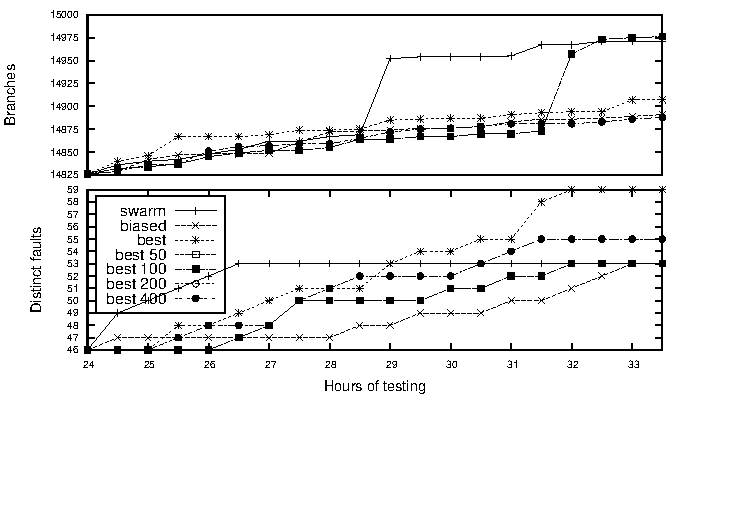
\includegraphics[width=\textwidth]{../graphs/SpiderMonkey/js16strats}
  \vspace{-1.3in}
  \caption{SpiderMonkey 1.6 Feedback Results}
  \label{fig:smonkey16strat}
\end{figure*}

\begin{figure*}
  \centering
  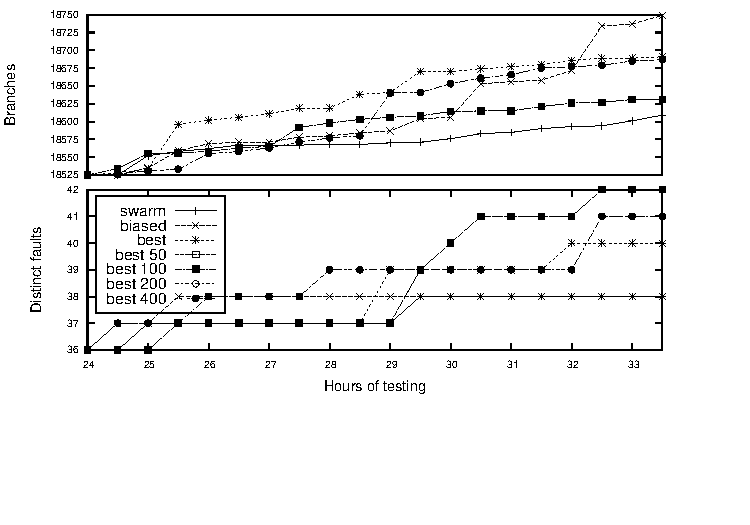
\includegraphics[width=\textwidth]{../graphs/SpiderMonkey/js17strats}
  \vspace{-1.5in}
  \caption{SpiderMonkey 1.7 Feedback Results}
  \label{fig:smonkey17strat}
\end{figure*}

Figures \ref{fig:smonkey16strat} and \ref{fig:smonkey17strat} show the
results of attempting to exploit the results of the first 24 hours of
swarm testing to improve testing for the next 24 hour period, tuning
the configurations used.  

Because measuring code coverage after each test is expensive, we used
a feedback approach based on coverage over difficult-to-execute
coverage entities only.  We considered a branch or line
``uninteresting'' if it was executed during every 30 minute run in the
first 24 hours of testing.  Coverage for the remaining ``interesting''
blocks and branches only was collected for each test, and
ranked configurations by the total value (the log of the inverse of
the frequency of coverage over all tests) of all covered entities.
The feedback strategies were then (1) to re-use the best (or best 50,
100, 200, or 400) configurations in round-robin fashion for future
test generation, and (2) to include each feature with a biased
non-50\% probability based on its frequency in tests executing at least
one interesting coverage entity.

While some strategies show a cumulative improvement on swarm in terms
of coverage or fault detection, \emph{no improvements} (measured in
terms of 30 minute run improvements on the cumulative swarm coverage
at 24 hours) are statistically significant; in some cases there was a
statistically significant \emph{reduction} in new distinct faults per
run.  The results were similar enough to the pure swarm strategy, and
required sufficient computational effort (in computing detailed
coverage results and ranking configurations) and additional test
infrastructure development that we find little support for applying
simple feedback mechanisms.  It is possible more sophisticated
methods, e.g. using machine learning, may be valuable, but the most
important goal would be to cover \emph{never-executed} code, for which
there is, in general, no data from which learn a good configuration.
Our hypothesis was that executing infrequently executed code more
often should lead to either detection of bugs concerning that code, or
execution of ``nearby'' uncovered code.  While feedback did indeed
increase the frequency of rarely executed entities, it did not produce
a clear effect in terms of bugs or novel coverage.
